\documentclass[a4paper, 12pt]{article}

%Paragraph jumps and indentation
\setlength{\parskip}{1.5em}
\setlength{\parindent}{1.25cm}

%Border
\usepackage[left=1in, right=1in, top=1in, bottom=1in]{geometry}

%Double spacing
\usepackage{setspace}
\doublespacing

%Packages
\usepackage{amsmath}
\usepackage[dvipsnames]{xcolor}
\usepackage{mathtools}
\usepackage{amsfonts}
\usepackage{titlesec}

%Images
\usepackage{graphicx}
\graphicspath{ {./images/} }
\usepackage{wrapfig}
\usepackage{float}

%Tables
\usepackage{multirow}
\usepackage{array}
\usepackage{tabu}
\titleformat{\section}
{\normalfont\large\bfseries}{\thesection}{1em}{}
\titleformat{\subsection}
{\normalfont\large\bfseries}{\thesubsection}{1em}{}

%Equation numbering
\counterwithin{equation}{section}

%Links
\usepackage{hyperref}
\urlstyle{same}

%Diagrams
\usepackage{pgfplots}
\pgfplotsset{compat=newest}
\usetikzlibrary{positioning, arrows.meta}
\usepgfplotslibrary{fillbetween}
\usepackage{wrapfig}


\begin{document}

\begin{titlepage}
  \begin{center}
    \textbf{IB ECONOMICS} \hspace{1cm} STANDARD LEVEL\\
    \vspace*{3cm}
    \textbf{Title of the article:}
    Yle budget cuts agreed after Left,
    Greens and Finns Party approve new deal\\

    \textbf{Source of the article:}
    Yle News\\

    \textbf{Link to the article:}
    \url{https://yle.fi/a/74-20111279}\\

    \textbf{Article publish date:}
    September 12, 2024\\

    \textbf{Article access date:} January 31, 2025\\

    \textbf{Commentary writing date:} January 31, 2025\\

    \textbf{Unit of the syllabus:}
    Microeconomics\\

    \textbf{Key concept:}
    Economic Well-Being.\\

    \vfill
    Word count: 731
  \end{center}
\end{titlepage}

\section*{Extract}
{ \itshape
  {\large The deal means that Yle faces a funding freeze and an increase in VAT payments, after a long drawn-out battle over setting the company's spending limits up to 2027.}

  Yle faces a years-long funding freeze after parliamentary parties agreed a deal on the company's budget, with the Finns Party, Greens and Left Alliance all approving the new agreement.

  The deal will freeze the budget until 2027, and increase the VAT rates levied on the company from 10 percent to 14 percent from 2026. Yle's budget in 2027 will be around 47 million euros smaller than it would be if index-linked budget increases occurred annually.

  The company will also be obliged to increase commissioning from external production companies, with external purchases slated to be around 15-20 percent higher than they were in the period 2021-2023.

  In addition, Yle will be required to publish more information about its activities and spending.

  The company is owned by the Finnish state and funded by a tax that in 2024 was a maximum of 163 euros per year for individual taxpayers, with reductions for those on lower incomes, or 3,000 euros for businesses.

  Parties have been at loggerheads over Yle's budget since the election campaign, in which both the National Coalition and Finns Party argued for cuts worth more than a hundred million euros in Yle's funding.
}
\newpage
\textbf{\textit{\large Consensus decision}}\\
{ \itshape

  Yle's budget is traditionally decided by cross-party consensus, separate to the government programme. This is regarded as a safeguard against politicising the public service media company, but this time around negotiations were difficult and protracted.

  National Coalition MP Matias Marttinen chaired the working group seeking a compromise, with his own party and the Finns Party suggesting that the government could take the decision themselves if cross-party consensus wasn't reached.

  In July a proposal was accepted by all the parliamentary parties except the Greens and the Left Alliance, who were annoyed at the way the proposal had been negotiated between the Finns Party and National Coalition, rather than between all the parties in the working group.

  The two parties secured small changes to the text of the deal, relating to working conditions of staff and reinforced a commitment to the production of high quality programming for children and young people, and its role as a pillar of general education and a guarantor of equality in educational equality.

  The Movement Now party, a one-man group consisting of Apprentice presenter Harry Harkimo, announced early on that it would reject the agreement on Yle funding.
}

\newpage

\section*{Commentary}

The article extols the conclusion of discussions within the government regarding the endowment of Yle, the Finnish Public Service Media Company.
Consensus is reached after much deliberation, and as a result the budget of Yle shall be diminished both directly, by reducing the direct tax "yleisradiovero" from 163\texteuro\ to 160\texteuro, and indirectly through the funding freeze and the VAT increase.
This commentary aims to analyse the effects of the changes by simplifying the situation and treating it as a reduction of direct provision to the news market by the government.
It shall be demonstrated that this change successfully advances \textbf{economic well-being}, around which the dialogue shall revolve.
To inspect the potential consequences of this modification, one must first discern the condition antecedent to the alteration.

\begin{wrapfigure}{L}{0.6\textwidth}
  \begin{center}
    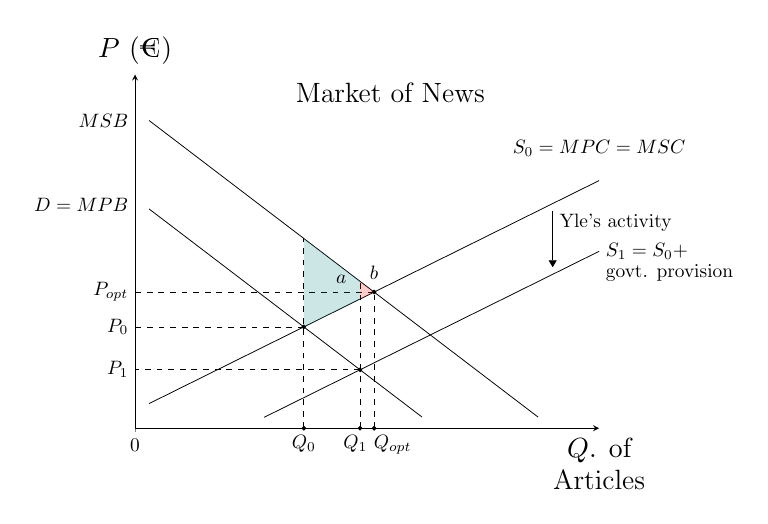
\begin{tikzpicture}[scale=0.7]
      \begin{axis}[
          width=10cm,
          height=8cm,
          axis lines=left,
          xtick={0},
          ytick={\empty},
          xmin=0, xmax=10,
          ymin=0, ymax=10,
          clip=false
        ]

        \addplot[domain=0.3:10, restrict y to domain=0.3:10, samples=400]{0.65*x+0.5};
        \addplot[domain=0.3:10, restrict y to domain=0.3:10, samples=400]{0.65*x-1.5};


        \addplot[domain=0.3:10, restrict y to domain=0.3:10, samples=400]{-x+6.5};
        \addplot[domain=0.3:10, restrict y to domain=0.3:10, samples=400]{-x+9};


        \node[above] at (10, 7.5) {$S_0=MPC=MSC$};
        \node[right] at (10, 5) {$S_1=S_0 + $};
        \node[right] at (10, 4.4) {govt. provision};

        \node[left] at (0, 6.3) {$D=MPB$};
        \node[left] at (0, 8.7) {$MSB$};

        \draw[dashed] (5.15152, 0) -- (5.15152, 3.84849);
        \draw[dashed] (0, 3.84849) -- (5.15152, 3.84849);
        \filldraw[black] (5.15152, 3.84849) circle (1pt);
        
        \filldraw[black] (5.15152, 0) circle (1pt);
        \node[below] at (5.55152, 0) {$Q_{opt}$};
        \node[left] at (0, 3.84848) {$P_{opt}$};
        
        \draw[dashed] (3.63636, 0) -- (3.63636, 5.36364);
        \draw[dashed] (3.63636, 2.86364) -- (0, 2.86364);
        \filldraw[black] (3.63636, 2.86364) circle (1pt);
        
        \filldraw[black] (3.63636, 0) circle (1pt);
        \node[below] at (3.63636, 0) {$Q_0$};
        \node[left] at (0, 2.86364) {$P_0$};


        \draw[dashed] (4.848, 0) -- (4.848, 4.152);
        \draw[dashed] (4.848, 1.652) -- (0, 1.652);
        \filldraw[black] (4.848, 1.652) circle (1pt);
        
        \filldraw[black] (4.848, 0) circle (1pt);
        \node[below] at (4.748, 0) {$Q_1$};
        \node[left] at (0, 1.652) {$P_1$};
        
        \fill[teal, opacity=0.2] (3.63636, 2.86364) -- (4.848, 3.651) -- (4.848, 4.152) -- (3.63636, 5.36364);
        \node[left] at (4.7, 4.2) {$a$};

        \fill[red, opacity=0.2] (5.15152, 3.84848) -- (4.848, 3.651) -- (4.848, 4.152);
        \node[above] at (5.15152, 4) {$b$};

        \draw[-Triangle] (9, 6.15) to (9, 4.55);
        \node[right] at (9, 5.8) {Yle's activity};

        \node[below] at (10, -1) {\Large Articles};
        \node[above] at (5.5, 9) {\Large Market of News};

      \end{axis}
      \node[below] at (current axis.right of origin) {$Q$. of};
      \node[above] at (current axis.above origin) {$P \text{ (\texteuro)}$};
    \end{tikzpicture}
    \caption{Introducing Yle to Reduce Welfare Loss}
  \end{center}
\end{wrapfigure}

\noindent \textbf{Figure 1} illustrates the externality that would arise were the Finnish government to abstain from intervening in the news markets through the direct provision of content via Yle.
When Finnish citizens consume news, it renders them more erudite and informed, thereby producing benefit to the whole society that the individual consumer is unaware of.
Consequently, the marginal social benefit ($MSB$) is greater than the marginal private benefit ($MPB$) at each quantity.
If the government does not intervene, the market equilibrium would rest at $(P_0, Q_0)$, meaning the quantity produced is inferior to $Q_{opt}$, the optimum quantity of News the Finnish market should be producing.
That means an unregulated market forgoes social surplus equal to the area $a+b$, so that is the amount of welfare loss occasioned by the positive consumption externality. 
The government undertakes direct provision in the News market by creating Yle, whose charge is to rectify the welfare loss.

The effects of introducing Yle to directly provide news increases the supply of news from $S_0$ to $S_1$.
The price and quantity of news settle to new equilibriums $P_1$ and $Q_1$ respectively.
This is favourable, as the welfare loss in this case is limited to area $b$, so the social surplus is increased by $a$.

\begin{wrapfigure}{L}{0.6\textwidth}
  \begin{center}
    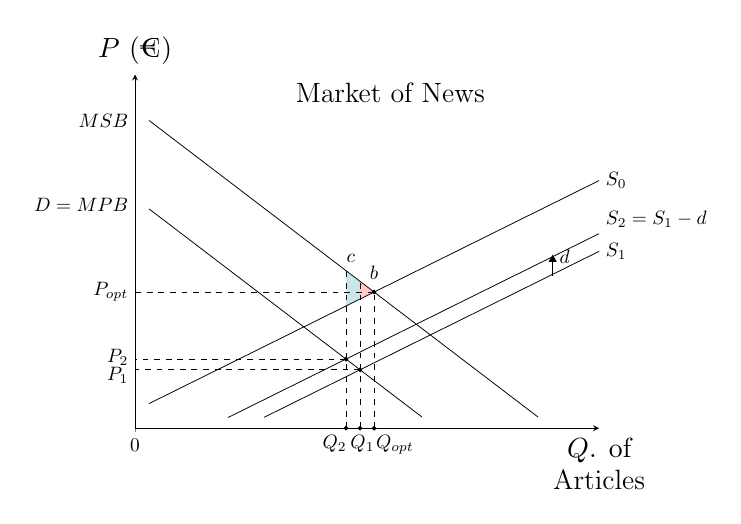
\begin{tikzpicture}[scale=0.7]
      \begin{axis}[
          width=10cm,
          height=8cm,
          axis lines=left,
          xtick={0},
          ytick={\empty},
          xmin=0, xmax=10,
          ymin=0, ymax=10,
          clip=false
        ]

        \addplot[domain=0.3:10, restrict y to domain=0.3:10, samples=400]{0.65*x+0.5};
        \addplot[domain=0.3:10, restrict y to domain=0.3:10, samples=400]{0.65*x-1};
        \addplot[domain=0.3:10, restrict y to domain=0.3:10, samples=400]{0.65*x-1.5};

        \addplot[domain=0.3:10, restrict y to domain=0.3:10, samples=400]{-x+6.5};
        \addplot[domain=0.3:10, restrict y to domain=0.3:10, samples=400]{-x+9};


        \node[right] at (10, 7) {$S_0$};
        \node[right] at (10, 5) {$S_1$};
        \node[right] at (10, 5.9) {$S_2=S_1-d$};

        \node[left] at (0, 6.3) {$D=MPB$};
        \node[left] at (0, 8.7) {$MSB$};

        \draw[dashed] (5.15152, 0) -- (5.15152, 3.84849);
        \draw[dashed] (0, 3.84849) -- (5.15152, 3.84849);
        \filldraw[black] (5.15152, 3.84849) circle (1pt);
        
        \filldraw[black] (5.15152, 0) circle (1pt);
        \node[below] at (5.6, 0) {$Q_{opt}$};
        \node[left] at (0, 3.84848) {$P_{opt}$};

        \draw[dashed] (4.848, 0) -- (4.848, 4.152);
        \draw[dashed] (4.848, 1.652) -- (0, 1.652);
        
        \filldraw[black] (4.848, 1.652) circle (1pt);
        \filldraw[black] (4.848, 0) circle (1pt);
        \node[below] at (4.9, 0) {$Q_1$};
        \node[left] at (0, 1.5) {$P_1$};

        \draw[dashed] (4.54545, 0) -- (4.54545, 4.45455);
        \draw[dashed] (4.54545, 1.95455) -- (0, 1.95455);
        \filldraw[black] (4.54545, 1.95455) circle (1pt);
        \filldraw[black] (4.54545, 0) circle (1pt);
        \node[below] at (4.3, 0) {$Q_2$};
        \node[left] at (0, 2) {$P_2$};


        
        \fill[red, opacity=0.2] (5.15152, 3.84848) -- (4.848, 3.651) -- (4.848, 4.152);
        \node[above] at (5.15152, 4) {$b$};

        \fill[teal, opacity=0.2] (4.54545, 3.45454) -- (4.54545, 4.45455) -- (4.848, 4.152) -- (4.848, 3.651);
        \node[above] at (4.65152, 4.5) {$c$};

        \draw[-Triangle] (9, 4.3) to (9, 4.9);
        \node[right] at (9, 4.85) {$d$};

        \node[below] at (10, -1) {\Large Articles};
        \node[above] at (5.5, 9) {\Large Market of News};

      \end{axis}
      \node[below] at (current axis.right of origin) {$Q$. of};
      \node[above] at (current axis.above origin) {$P \text{ (\texteuro)}$};
    \end{tikzpicture}
    \caption{Effects of the Budget Cut}
  \end{center}
\end{wrapfigure}

\noindent The budget cut is illustrated in \textbf{Figure 2} as a reduction in the supply of news, by some amount $d$ which will be discussed later.
The change means market equilibrium will now be at $(P_2, Q_2)$, and an additional welfare loss equal to $c$ will be borne.

We wish to assess the magnitude of loss, and for completeness we will first discuss a factor not accounted for in the diagram.
The fact that there is a lower quantity or quality of perfectly impartial news supplied by the government means the size of marginal social benefit may contract to some degree.
This arises because other news outlets in the market might be aligned with political factions or less devoted to serving the populace compared to Yle, prioritising their pecuniary gains instead.

An important note is that the magnitude of the change may not be as pronounced as the diagram suggests.
This is because the cut is made to the company's budget, so its effects are distributed over all of Yle's activities. 
For example, we may expect the company to be producing less sports commentary or entertainment programmes, instead of sacrificing the quantity or quality of news provided.

The speculations above are too vague, and a production possibilities curve (PPC) will be used to obtain a better idea of the specifics.
The article states that the budget will shrink by approximately $47$ million euros, or $\approx 8.6\%$\footnote{The total budget was $547$ million euros in 2024, according to \url{https://yle.fi/a/74-20117417}}.

\begin{wrapfigure}{L}{0.6\textwidth}
  \begin{center}
    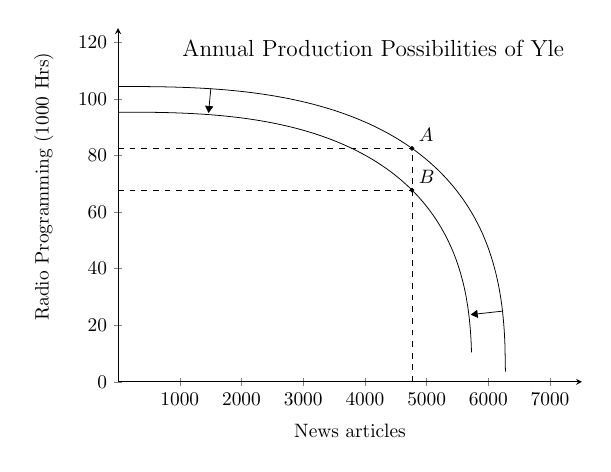
\begin{tikzpicture}[scale=0.7]
      \begin{axis}[
          width=10cm,
          height=8cm,
          axis lines=left,
          xtick={1.33,2.66,...,10},
          xticklabels={1000,2000,...,7000},
          ytick={0,1.6,...,9.6},
          yticklabels={0,20,...,120},
          xmin=0, xmax=10,
          ymin=0, ymax=10,
          clip=false
        ]
        
        \addplot[domain=0:10, restrict y to domain=0:10, samples=1000] {(320-x^2.71828)^0.367879};
        \addplot[domain=0:10, restrict y to domain=0:10, samples=1000] {(250-x^2.71828)^0.367879};

        \draw[-Triangle] (2, 8.3) to (1.95, 7.6);
        \draw[-Triangle] (8.3, 2) to (7.6, 1.9);
        %\draw[-Triangle] (6, 6) to (5.5, 5.4);

        \draw[dashed] (0, 6.6) -- (6.3337, 6.6);
        \draw[dashed] (6.3337, 0) -- (6.3337, 6.6);
        \draw[dashed] (0, 5.42086) -- (6.3337, 5.42086);

        \filldraw[black] (6.3337, 6.6) circle (1pt);
        \node[above right] at (6.3337, 6.6) {$A$};

        \filldraw[black] (6.3337, 5.42086) circle (1pt);
        \node[above right] at (6.3337, 5.42086) {$B$};
        
        \node[below] at (5, -1) {News articles};
        \node[left, rotate=90] at (-1.6, 9.5) {Radio Programming (1000 Hrs)};
        \node[above] at (5.5, 9) {\large Annual Production Possibilities of Yle};

      \end{axis}
    \end{tikzpicture}
    \caption{Change in the PPC of Yle}
  \end{center}
\end{wrapfigure}

\noindent \textbf{Figure 3} shows the reduction in Yle's production possibilities, and the choice it must face between producing radio programming and making news available.
We define availability as a measure influenced by quantity, quality, and the topicality of the news.
In 2023, the amount of radio programming produced is $82,210$ hours\footnote{\url{https://yle.fi/aihe/ylen-vuosi-2023}}, as reflected by the diagram.
According to this illustration, this corresponds to producing $48,000$ articles\footnote{This is my estimate on the number of articles published in a year, since no official data is available.}.
To avert compromising \textbf{economic well-being} through providing less news, Yle may strive to maintain it constant.
That would entail reducing radio programming to about $69,000$ hours.

If this course were adopted, the news market would face no change, so $d\approx0$, and equivalently the additional welfare loss $c$ would not be incurred.
Additionally, the size of the positive consumption externality would not decrease, avoiding further losses.
I believe this is the most probable outcome since radio programmes (particularly entertainment) generally yield less positive externalities compared to news.
The government and Yle by extension strive for \textbf{economic well-being}, and thus wish to accord precedence to benefits in the long run.

\end{document}